
\documentclass[letterpaper,12pt]{memoir}
\newsavebox{\FrontImgBox}
\newlength{\FrontClip}
\usepackage{float}



\usepackage[pdftex]{graphicx}
%block size info
\settypeblocksize{7.25in}{4.5in}{*}
\addtolength{\textheight}{\onelineskip}
\setlrmargins{2.1in}{*}{1}
\setulmargins{1.75in}{*}{1}
\checkandfixthelayout
\usepackage{todonotes}
\pagestyle{empty} % no page number
\usepackage[pdftex]{graphicx}
\usepackage{eso-pic}

\settypeblocksize{7.25in}{4.5in}{*}
\addtolength{\textheight}{\onelineskip}
\setlrmargins{2.1in}{*}{1}
\setulmargins{1.75in}{*}{1}
\checkandfixthelayout
 \usepackage{microtype} % better justification & protrusion
\usepackage{newtxtext} % Times-like body text (newspaper vibe)
\usepackage[scaled]{helvet} % Sans for headlines and decks
\usepackage[T1]{fontenc}
\usepackage[utf8]{inputenc}

% ====== Columns & visuals ======
\usepackage{multicol}
\setlength{\columnsep}{0.28in}
\setlength{\columnseprule}{0.2pt}

\usepackage{graphicx}
\usepackage{wrapfig}
\usepackage{caption}
\captionsetup{font=small,labelfont=bf}

\usepackage[dvipsnames]{xcolor}
\usepackage{lettrine} % drop caps
\usepackage[many]{tcolorbox} % pull quotes / sidebars
\usepackage[print,1to1]{booklet} %print option switches to landscape
\pagespersignature{16}
\usepackage{pgfplots}
\pgfplotsset{width=10cm,compat=1.9}

\tcbset{
  colback=black!2,
  colframe=black!40,
  boxsep=4pt, left=6pt, right=6pt, top=6pt, bottom=6pt,
  sharp corners,
}

% ====== Headings & bylines ======
\setsecheadstyle{\Large\bfseries\sffamily}
\setsubsecheadstyle{\normalsize\bfseries\sffamily}
\setsubsubsecheadstyle{\normalsize\itshape}

\newcommand{\kicker}[1]{\textsf{\bfseries\small\color{Gray} #1}}
\newcommand{\headline}[1]{\textsf{\bfseries\fontsize{34}{36}\selectfont #1}}
\newcommand{\deck}[1]{\textsf{\large\itshape #1}}
\newcommand{\byline}[1]{\textsf{\small\color{Gray} Af #1}}
\usepackage{tikz}
\usetikzlibrary{fadings,patterns}

% Define a generic "fade to transparent" around a rectangle
\tikzfading[name=image fade,
  inner color=transparent!50,
  outer color=transparent!100]

  % Text outline ("border around letters")
\usepackage{contour} % works with pdfLaTeX/XeLaTeX/LuaLaTeX
\contourlength{0.9pt}         % default stroke thickness
\contournumber{32}            % smoothness of the outline

% Helpers: white text with dark outline (and a thinner variant)
\newcommand{\ow}[2][black]{\contour{#1}{\textcolor{white}{#2}}}
\newcommand{\owthin}[2][black]{%
  \begingroup\contourlength{0.6pt}\contour{#1}{\textcolor{white}{#2}}\endgroup}

% ====== Page banner / folio ======
\makepagestyle{newspaper}
\makeoddhead{newspaper}{\textsf{\small Den Rullende Sten}}{}{\textsf{\small Sponsoreret af Det Glemte Akademi}}
\makeevenhead{newspaper}{\textsf{\small Sponsoreret af Det Glemte Akademi}}{}{\textsf{\small Den Rullende Sten}}
\makeoddfoot{newspaper}{}{\textsf{\small\thepage}}{}
\makeevenfoot{newspaper}{}{\textsf{\small\thepage}}{}
\makeheadrule{newspaper}{\textwidth}{0.4pt}
\pagestyle{newspaper}

% ====== Pull quote and sidebar environments ======
\newenvironment{pullquote}
  {\begin{tcolorbox}[enhanced, breakable]\itshape\large}
  {\end{tcolorbox}}


\usepackage{xparse}
\usepackage{wrapfig}

% Justérbare standarder for sidebar i spalter
\newcounter{sidebarlines}              % hvor mange linjer der skal "wrappe" forbi boksen
\setcounter{sidebarlines}{14}
\setlength{\sidebarwidth}{0.42\columnwidth}


% ====== Utilities ======
\newcommand{\separator}{%
  \par\noindent{\color{black!40}\rule{\textwidth}{0.4pt}}\par
}


% Front feature image: spans \textwidth, keeps aspect ratio, fades at edges,
% and overlays outlined text (no boxes).
% Usage: \FrontFeatureImage{<image>}{<kicker>}{<headline>}{<deck>}{<credit>}
\newcommand{\FrontFeatureImage}[5]{%
  % Typeset image at \textwidth just once and measure its height
  \sbox{\FrontImgBox}{\includegraphics[width=\textwidth]{#1}}%
  % Total height of the scaled image (height + depth)
  \dimen0=\dimexpr\ht\FrontImgBox+\dp\FrontImgBox\relax
  % Max allowed height
  \dimen2=.75\textheight
  % Choose visible height: min(actual, max)
  \ifdim\dimen0>\dimen2
    \setlength{\FrontClip}{\dimen2}%
  \else
    \setlength{\FrontClip}{\dimen0}%
  \fi
  %
  \begin{tikzpicture}
    % Define a "frame" we’ll use for anchors & clipping
    \coordinate (TL) at (0,0);                       % top-left
    \coordinate (TR) at (\textwidth,0);              % top-right
    \coordinate (BL) at (0,-\FrontClip);             % bottom-left (cropped)
    \coordinate (BR) at (\textwidth,-\FrontClip);    % bottom-right (cropped)

    % Image with soft fading edges, clipped to the frame (crops from the bottom)
    \begin{scope}
      \clip (TL) rectangle (BR);
      \node[anchor=north west, inner sep=0pt,
            path fading=image fade, fit fading=false] at (TL)
        {\usebox{\FrontImgBox}};
    \end{scope}

    % Dark wash for legibility, also softly faded (match the same clip)
    \begin{scope}
      \clip (TL) rectangle (BR);
      \fill[black,opacity=0.30, path fading=image fade] (BL) rectangle (TR);
    \end{scope}

    % Text stack (bottom-left) — outline style preserved
    \node[anchor=south west, xshift=1em, yshift=1em, align=left,
          text width=.75\textwidth] at (BL){%
      \sffamily
      % Kicker (optional)
      \if\relax\detokenize{#2}\relax\else
        {\owthin[black!85]{\textsf{\bfseries\small #2}}}\\[0.15em]\fi
      % Headline
      {\ow{\bfseries
        \resizebox{1\textwidth}{!}{#3}%
      }}\\[0.2em]
      % Deck
      {\owthin{\large\itshape #4}}%
    };

    % Credit (bottom-right), small outline
    \node[anchor=south east, xshift=-1em, yshift=1em] at (BR)
      {\sffamily\small \owthin[black!85]{#5}};
  \end{tikzpicture}%
}



 

\begin{document}
\pdfpageheight=\paperwidth
\pdfpagewidth=\paperheight
\paperwidth=\pdfpagewidth
\paperheight=\pdfpageheight 
% ====== Nameplate ======
\begin{figure}
  \begin{center}
      
\includegraphics[width=0.98\textwidth]{Logo.png}%
  \end{center}    
\end{figure}
\begin{center}
  {\Large\sffamily Udgave 131}
\end{center}


% Front feature image (keeps aspect ratio, spans \textwidth)
\FrontFeatureImage{Skriveren.png}
{Skriveren observeret i A'kastin}
{Hvad betyder det for Imperiets økonomi?}
{Vil alle guderne overleve?}
{}

\vspace{.75\baselineskip}


% ====== Lead story (Front page) ======
\par\medskip
\headline{En ny hånd i skyggerne}
\par\medskip
\deck{Johannes Krell set i A’kastin.}
\par\medskip
\byline{Redaktionen}
\medskip

\lettrine[lines=3,lhang=0.1,loversize=0.05]{D}{et} begyndte som hvisken i kroer og blandt skriftkloge: en fremmed mand, set i A’kastin, mange har rapporteret at han har sat telt op uden for Marcusstad. Gennem vores journalister i felten har vi opnået bekræftelse: Johannes Krell er den nye Skriver. Men hvem er Skriveren egentlig?

\par\medskip

I de lævn af sagn vi har fundet er Skriveren en kosmisk funktion, men mod hvem vides ikke.

Historisk set opstod Skriveren efter den såkaldte Tavse Splittelse, hvor flere lærde forsøgte at samle skrifter om en ukendt overgud og gik fra forstanden. Det siges, at Skriveren har to artefakter: Skriverens bog, hvor al viden står beskrevet, samt Skriverens pen, som gør alt hvad der skrives med den til virkelighed.

\par\medskip

Men hvem er så Johannes Krell? Det spørgsmål er langt sværere. Officielt er han en lavadelig akademiker fra Imperiets nordlige provinser. Men han er kendt for værker som I akademiske kræse beskrives som værende "Af varierende standard".

Flere vidner beskriver ham som rolig.

Andre peger på hans tidligere værker, særligt den berygtede bog \emph{“Guder og dig”}, hvor han udfordrede selve definitionen af guddommelighed. En bog der i årevis blev latterliggjort, og nu pludselig læses med ny alvor.

\begin{pullquote}
“Vi troede han var fuld, ja vi gav ham endda tilnavnet den Fulde Præst. Det viser sig, at han måske bare var foran os.”
- Kelllwan Biskob Magnus Finkelborg
\end{pullquote}

\par\medskip

Dette bringer os til et mere jordnært, men ikke mindre vigtigt spørgsmål: \emph{Hvad betyder det for Imperiets økonomi?}

Hvis blot en brøkdel af legenderne er sande, står vi over for en magt, der kan omskrive virkeligheden selv. Hvad sker der med handel, hvis efterspørgelse kan slettes med et ord? Hvad sker der med gæld, hvis den kan skrives bort?

Markeder er bygget på tillid, men også på begrænsninger. Skriveren repræsenterer noget langt farligere: en verden uden begrænsninger.

\par\medskip

Men økonomi er intet i forhold til det næste spørgsmål: \emph{Vil alle guderne overleve?}

Hvis Krells egne teorier holder stik, afhænger gudernes styrke af tilbedelse. Hvis virkeligheden selv kan ændres, hvad sker der så med troen?

\par\medskip

Der er dog nogen som siger at Skriveren ikke har adgang til sin pen, men i stedet har et kort over hele Kalish. Hvad dette betyder og hvordan dette påvirker verdenen er usikkert, men det kunne være en forklaring for den politiske udvikling vi har set i de sidste måneder. 

\section*{Nyheder}
\subsection*{A'kastin indsamler til ny port}
\textit{- Gert Günther Gammelgaard}\\
\begin{tikzpicture}
\begin{axis}[
    ybar,
    ymin=0,
    ymax=100,
    bar width=18pt,
    symbolic x coords={Jern,Mitril,Runer,Fjend},
    xtick=data,
    x tick label style={rotate=45, anchor=east},
    ytick={0,20,40,60,80,100},
    yticklabel style={
        /pgf/number format/1000 sep=
    },
    ylabel={Procent},
    enlargelimits=0.15,
    width=10cm,
    height=7cm,
    legend style={
        at={(0.5,-0.22)},
        anchor=north,
        legend columns=-1
    },
]
\addplot coordinates {
    (Jern,11)
    (Mitril,1.25)
    (Runer,0)
    (Fjend,7.32)
};
\legend{Marts}
\end{axis}
\end{tikzpicture}
\newline 
A'kastin har været ved at samle ressourcer ind til en ny port. De lader til at have bestemt sig for at gøre dette selv, og på trods af at de har gjort stort og flot fremskridt så halter det stadig en smule.

På nuævrende tidspunkt har de indsamlet 11 ud af 100 Jern (11\%), 1 ud af 80 Mitril (1.25\%), 0 ud af 40 runer (0\%) og 293 ud af 4000 Fjend (7.32\%). 

Vi ønsker dem alt det bedste, og håber de får samlet deres ressourcer i tide.

\section*{Politik}
\subsection*{Debatindlæg: Omdøb Marcusstad til Dorianborg}
\textit{- Philip Kik}\\

Det er på tide, at vi tager stilling til, hvem vi ønsker at ære i vores samtid. Fortidens navne eller nutidens handlinger? Derfor bør Marcusstad omdøbes til Dorianborg, til ære for Dorian Vinterkrone.

Marcusstad bærer navnet på en fjern fortidsfigur, Kong Marcus, hvis betydning i dag mest er historisk og symbolsk. Men vi lever ikke i fortiden. Vi lever i en tid, hvor riger falder, dæmoner presser grænserne, og hvor handling vejer tungere end arv. Her har Dorian Vinterkrone bevist sit værd.

Han stod alene, da andre tøvede. Han sikrede Sydland, beskyttede handelsruter og skabte stabilitet, mens imperiet diskuterede. Fet er ansvar og lederskab i sin reneste form. Hvis en by skal bære et navn, bør det være en, der faktisk har kæmpet for dens borgere.

\begin{pullquote}
“Navne er valg vi tager. Og vi bør vælge dem, der stadig kæmper for os.”
— Gert Günther Gammelgaard
\end{pullquote}

Modstandere vil sige, at navnet Marcusstad er en del af vores kulturarv. Men kultur er ikke statisk. Den udvikler sig med de helte, vi vælger at hædre. Ved at omdøbe byen sender vi et klart signal: Vi værdsætter de helte der går blandt os i dag, og vi sætter mod over tradition.

Dorianborg vil være et symbol på en tid, hvor én mand gjorde det, andre ikke turde.

Spørgsmålet er derfor ikke, om vi skal ændre navnet.

Spørgsmålet er: Hvorfor har vi ikke gjort det endnu?
\par\medskip
\subsection*{Problemer ved græsen mellem Letho og Imperiet}
\textit{- Dagmar Hjulmølle}\\
I Skovbrynet syd for Nordland er der i de seneste uger blevet observeret et mærkeligt fænomen, som hverken jægere eller druider kan forklare. 
\par\medskip
Træerne står urørte, men deres skygger bevæger sig, selv når solen står stille. Flere rejsende beretter om hviskende stemmer, der ikke synes at tilhøre nogen levende skabning, og én handelsmand hævder at have fulgt sin egen skygge i flere timer, før den pludselig forsvandt. 
\par\medskip
Lokale myndigheder har endnu ikke udstedt en officiel forklaring, men enkelte lærde spekulerer i, om vi er vidner til en ny form for naturmagi eller noget langt ældre, som først nu er begyndt at røre på sig igen.
\par\medskip
Samtidig er grænsevagter fra både Imperiet begyndt at rapportere om uregelmæssigheder langs patruljeruterne. Spor forsvinder brat, som om de aldrig har eksisteret, og flere vagter har beskrevet en fornemmelse af at blive iagttaget uden at kunne finde kilden. 
\par\medskip
I et enkelt tilfælde vendte en patrulje tilbage med én mand i overskud. 
\par\medskip
Episoden er siden blevet fortiet officielt, men rygterne breder sig, og spændingerne langs grænsen er mærkbart tiltaget.
\newpage
\section*{Reklamer}
\subsection*{BRING JERN! OG KRUDT!}
\begin{figure}[H]
  \centering
  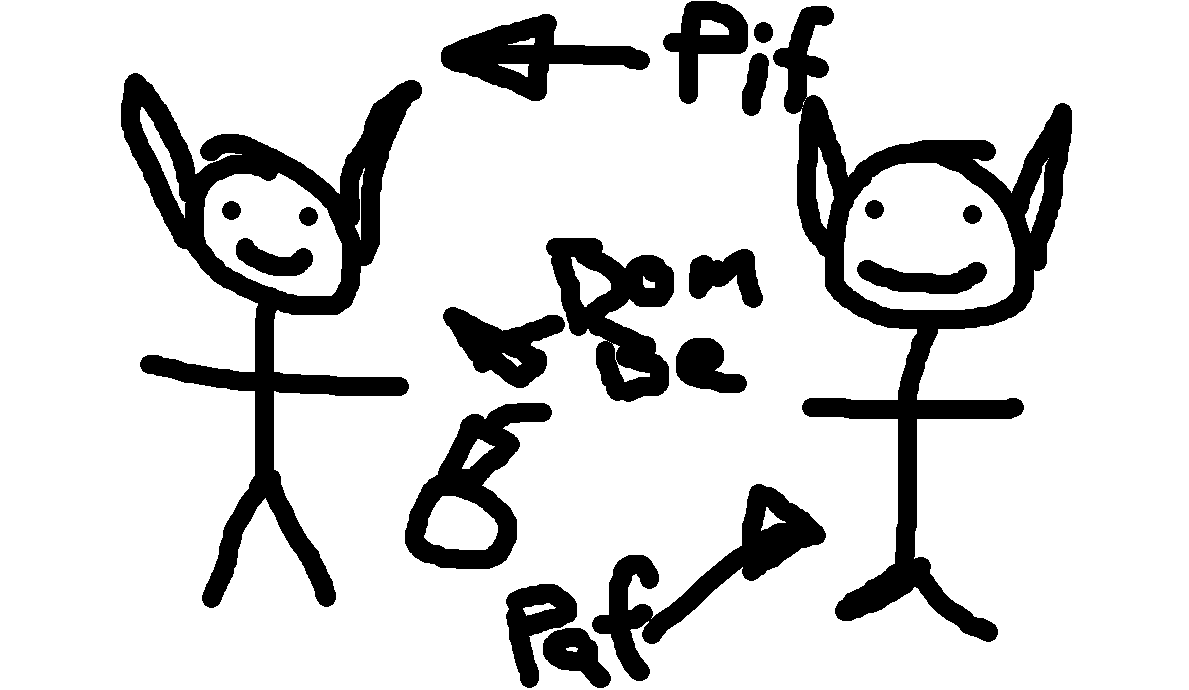
\includegraphics[width=0.9\textwidth]{PIFPAF.png}
\end{figure}
VI BRUG FOR KRUDT OG JERN TIL SPRINGE EVLER OP! DU BRING OS 5 JERN OG 5 KRUDT OG VI GIVE DIG SPECIEL PREMIE! DET VÆRE BOMBE I BREV! 
- PIF OG PAF!
\subsection*{Bliv rig uden at arbejde!}

Handelskompagniet giver dig en \textbf{eksklusiv mulighed} for at blive rig uden at løfte en finger! \\[0.5em]

Tjen op til \textbf{500 Fjend per dag}! \\[0.5em]

Alt du skal gøre, er at samle \textbf{Kongetand}! Handelskompagniet opkøber i øjeblikket alle de kongetand, vi kan få fat i. \\[0.5em]

Når du har bevist, at du kan samle 3 kongetand, får du \textbf{eksklusive rettigheder} til at oprette dit eget indsamlingskompagni! \\[1em]

\textit{Sådan fungerer det:}
\begin{itemize}
  \item Du samler 3 kongetander.
  \item Du finder 3 venner, der arbejder under dig.
  \item Hver af dem samler 3 kongetand til dig. Du har nu 9!
  \item Når de finder 3 venner hver, får du hele 36 kongetand!
\end{itemize}

Med vores atraktive handelsrate tilbyder vi \textbf{5 HKG}\footnote{Handelskompagni Guld} per kongetand. \\[0.5em]

Beviser du dit værd, bliver du udpeget til at være den officielle \textit{"Viceformand for eksklusiv kongetandsdistribution og indsamling"}.\footnote{Bevis for denne titel koster 5000 HKG eller 50 Fjend.} \\[1em]

\textbf{Kontakt din lokale repræsentant for Handelskompagniet i dag!}

\separator
% ====== Back matter (optional) ======
\section*{Kontakt}
Redaktionen, 1864 Salezstad

Ønsker du en artikel i Den Rullende Sten er det altid muligt at betale 15 Fjend for en 1 sides artikel.

\begin{figure}[H]
  \centering
  
\includegraphics[width=0.9\textwidth]{vinterkroneSkjold.png}
\end{figure}
Vi takker Familien Vinterkrone for deres støtte til Avisen.
\end{document}